\section{Q3. Reducing the risk that the model checker is incorrect}
%Does the report clearly describe what has been done to reduce the risk that the model checker is incorrect? Which parts of the explanation are good? Which parts could be improved and how?

In order to reduce the risk of the model checker to be incorrect, but still keep the implementations efficient, the formulae are implemented as follows:\\

The formulae \texttt{ctlTT}, \texttt{ctlNOT} and \texttt{ctlAND} are trivial, and not explained in depth. In general, inputs and outputs of the ctl methods should represent sets of states. This was implemented by storing the input states and output states in LinkedLists. The methods perform checks to avoid duplicates when necessary. 

\subsection{ctlEX}
EX = Exist neXt. This method returns all states which are able to reach at least one of the input states after one transition. \\

This was implemented in Java by looping through all states in the transition system, following the transitions to the target using \texttt{state.targets}, and checking whether the current target is contained in the input list if states.

\subsection{ctlAX}
AX = All neXt. Returns all states which are certain to reach one of the input states after one transition. \\

This was implemented in Java much like ctlEX, but additionally updating a boolean during each target evaluation:

\begin{lstlisting}
for (int target : state.targets) {
	check &= stateNrs.contains(target); 
}
if (check && state.targets.size() >= 1)
    matches.add(state);
\end{lstlisting}
The boolean \texttt{check} has the value \texttt{true} if the current examined state is in the represented in the input list of states, and \texttt{false} otherwise. If all condition-checks evaluated to true (using the \&= syntax) and the state has at least one edge, the examined state is added to the output list.

\subsection{ctlEF}
\label{sec:ctlEF}
EF = Exist Future. Returns all states which are able to reach at least one of the input states in an arbitrary amount of transitions. \\

This was implemented in Java by using a sort of \textbf{back propagation}. Each state has a boolean field \texttt{visisted}. Initially, this field contains the value \texttt{false}.\\

The list of output states is obtained using the following back propagation:
\begin{enumerate}
    \item All the input states are added to the output list of states, since the input states can reach the input states after 0 transitions.
    \item In a special for loop with increasing size, go through all states in the transition system. The loop size is mutated, but has an upper bound equal to the number of states in the transition system.
    \item If the examined state can reach a state in the \textbf{current} list of output states, \textbf{and it is not already added}, the state is added to the output list of states. The boolean used to check if the state is already added to the output list of states, is the \texttt{visited} boolean.
\end{enumerate}

The critical part of this method is the code snippet below:

\begin{lstlisting}
for (int i = 0; i < matches.size(); i++) {

	// go through all states in the TS
	for (State state : this.states) {

		if (state.targets.contains(matches.get(i).stateNr) && !state.visited) {
			matches.add(state);
			state.visited = true;
		}
	}
}
\end{lstlisting}

The output list matches has a maximum size equal to the number of states in the system, since each state can only be set to visited once. In particular, the loop condition \texttt{i $<$ matches.size()} demands some explanation. \\

If a transition system has $N$ states, each path fragment without a loop can at most be $N$ transitions long. The implementation of the outer for loop is built on this idea.\\

In the first run of the outer \text{for}-loop, all states in the transition system that can reach the \underline{input states} in one transition are added to the output. The loop size is increased, since the output list matches has increased in size.\\

In the next run of the outer \text{for}-loop, all states in the transition system that can reach one of the \underline{current output states} in one transition are added to the output.

\begin{figure}[H]
    \centering
    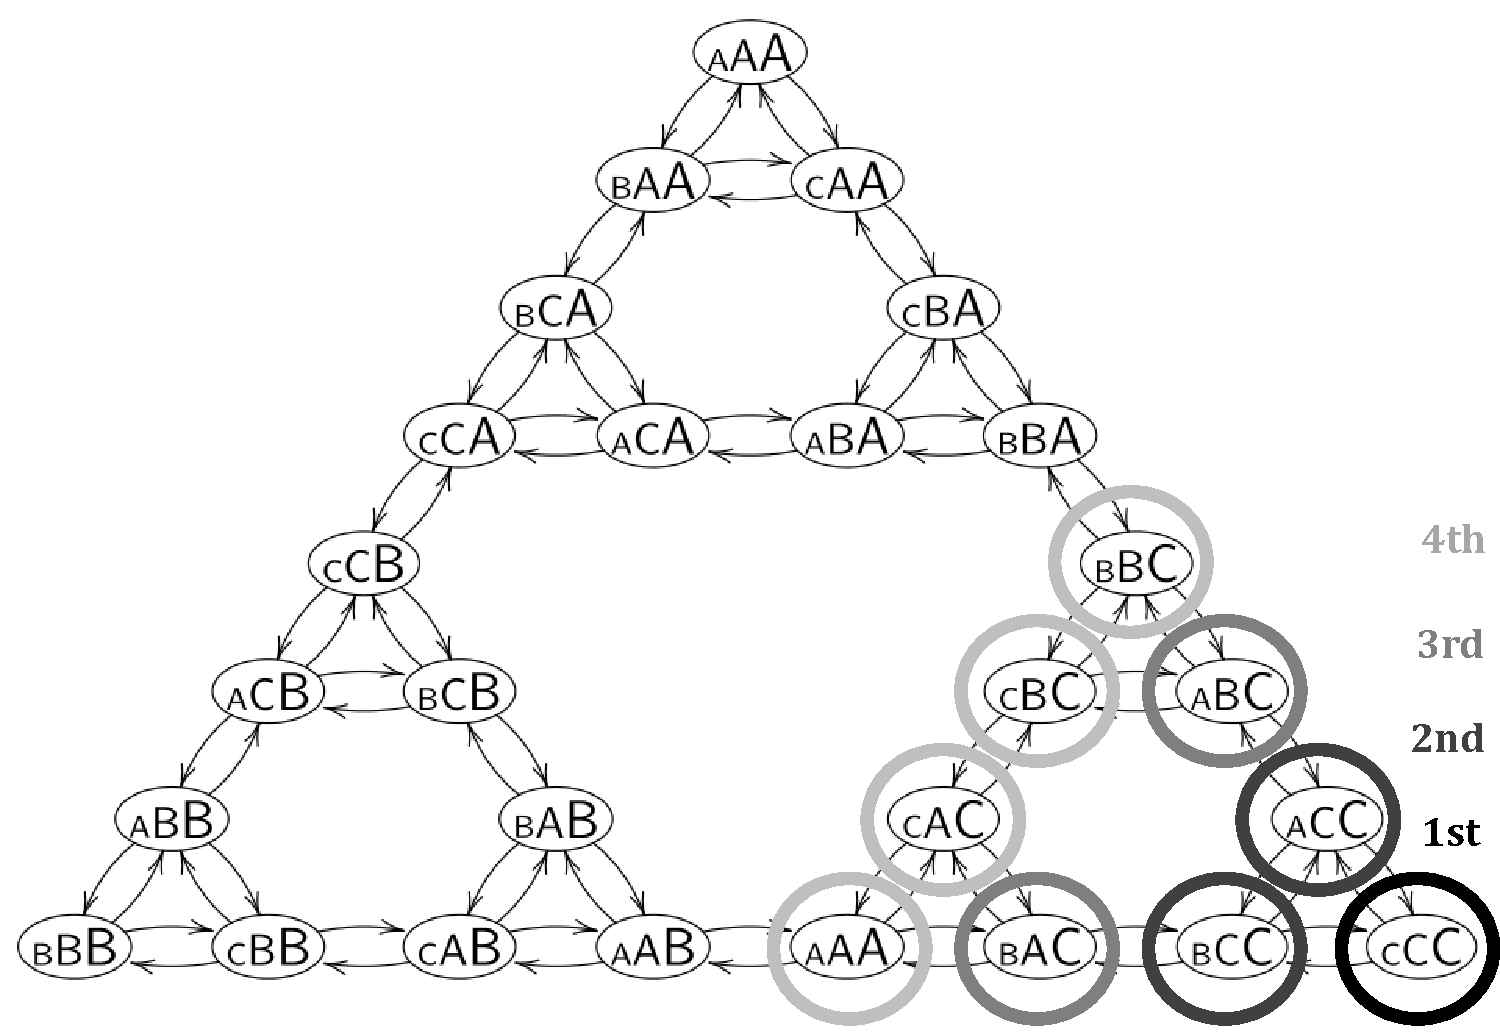
\includegraphics[width=0.8\textwidth]{fig/backprop.pdf}
    \caption{States found using ctlEF method with argument ctl CCC, during the first few steps of the outer for-loop of backward propagation.}
    \label{fig:backprop}
\end{figure}

\subsection{ctlAF (challenge)}
AF = All Future. This was implement using only few lines of Java code, and relied on our implementation of the ctlEG method:

\begin{lstlisting}
public List<State> ctlAF(List<State> satPhi) {
  return invertSet(ctlEG(invertSet(satPhi)));
	}
\end{lstlisting}

The intuition behind the implementation is the following:\\

For a given state in the input:
\begin{itemize}
    \item If all futures lead to satisfying $\phi$ for a given state, this state should be returned by \texttt{ctlAF}.
    
    \item If there exists an arbitrarily long path which you can avoid satisfying $\phi$, this state should not be returned by \texttt{ctlAF}.
\end{itemize}

Hence the all states fall into the following categories:

\begin{itemize}
    \item States for which futures lead to $\Phi$.
    
    \item States for which there exists an arbitrarily long path which you can avoid enjoying $\Phi$.
\end{itemize}

All states fall into one of the two categories above, so a more verbose way to describe the first category is by negating the second category:

\begin{enumerate}
    \item Find the states that can stay on paths satisfying $\neg \Phi$, using \texttt{ctlEG(invertSet(satPhi))}. These states correspond to category 1.
    \item Invert the found set of states using \texttt{invertSet(...)}. These states correspond to category 2. 
\end{enumerate}


\subsection{ctlEG (challenge)}
EG = Exist Global.
Returns all states which are able to stay in the set of given states for an arbitrarily long path. \\

The implementation corresponds to the description in section 5.5, page 183 in the notes, i.e. by using the auxiliary function \textt{F} and code corresponding to recursive function \texttt{iter}.

\begin{figure}[H]
    \centering
    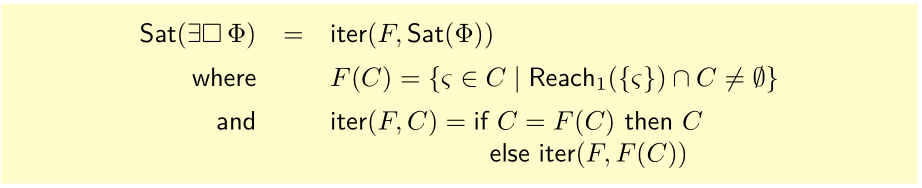
\includegraphics[width=1.0\textwidth]{fig/EG_def.PNG}
    \caption{The states that should returned by ctlEG, using page 183 in the notes.}
    \label{fig:EG_def}
\end{figure}


\begin{lstlisting}
public List<State> ctlEG(List<State> satPhi) {
  List<State> C = F(satPhi);

  // begin iter(F,C)
  // if C is stable under F, return C
  if (C.containsAll(satPhi) && (C.size() == satPhi.size())) {
    return satPhi;

  } else {
    // recurse
    return ctlEG(C);
  }
  // end iter(F,C)
}
\end{lstlisting}

In the note, the recursion occurs through the function \textt{iter}. In the Java implementation above, the functionality of \texttt{iter} is integrated into the \texttt{ctlEG} method, so the recursion occurs through \texttt{ctlEG}.

\subsection{ctlAG}
AG = All Global. Return all states which cannot escape the given list of states after an arbitrary number of transitions.\\

To avoid infinite loops, the implementation of the \texttt{ctlAG} method makes use of the \texttt{visited} field for each state.\\

For each state in the transition system, the auxiliary recursive method \texttt{chkAG} is called. 
Some terminology: States in the input are referred to as legal states. The remaining states are illegal. \\

The functionality is split into two methods:  \texttt{ctlAG} and \texttt{chkAG}.

\subsubsection{ctlAG}
\texttt{ctAG} loops over each state in the transition system, calls \texttt{chkAG}, adds the examined state to the output if \texttt{chkAG} returns true, and resets the visited fields between each \texttt{chkAG} call. The crucial part of of the \texttt{ctlAG} method is the following loop:

\begin{lstlisting}
for (State state : this.states) {

  // set visited field to false for all states
  resetVisit();

  // use a recursive auxiliary method
  if (chkAG(state, stateNrs))
    matches.add(state);
}
\end{lstlisting}

\subsubsection{chkAG}
\texttt{chkAG} determines whether the current state, or any targets after an arbitrary number of transitions, are illegal. This is achieved using \&= in Java; if just one target (after a number of transitions) is not legal, the boolean evaluates to false. \\

But which states should be checked by \texttt{chkAG}? Only those that have not been visited by the auxiliary method already.\\

\begin{lstlisting}
private boolean chkAG(State state, List<Integer> stateNrs) {

  // avoid duplicates
  if (!state.visited) {

    // if examined state is contained in input states
    if (stateNrs.contains(state.stateNr)) {
    state.visited = true;

    boolean check = true;
    for (int target : state.targets)
					
      // recursive: if a target is not legal, check evaluates to false
      check &= chkAG(get(target), stateNrs);

      return check;

    } else
    // if the state is visited for the first time, but not legal
    return false;

  } else
    // if the state has been visited already
    return true;
}
\end{lstlisting}





















